\documentclass[a0,portrait]{a0poster}

\usepackage[hidelinks]{hyperref}
\usepackage{multicol} % This is so we can have multiple columns of text side-by-side
\columnsep=100pt % This is the amount of white space between the columns in the poster
\columnseprule=3pt % This is the thickness of the black line between the columns in the poster

\usepackage{graphicx}
\usepackage{subfig}
\usepackage{fixltx2e}
\usepackage{wrapfig}

\usepackage[spanish, es-tabla]{babel}
\usepackage[utf8]{inputenc}

\usepackage[svgnames]{xcolor} % Specify colors by their 'svgnames', for a full list of all colors available see here: http://www.latextemplates.com/svgnames-colors

\usepackage{times} % Use the times font
%\usepackage{palatino} % Uncomment to use the Palatino font

\usepackage{graphicx} % Required for including images
\graphicspath{{figures/}} % Location of the graphics files
\usepackage{booktabs} % Top and bottom rules for table
\usepackage[font=small,labelfont=bf]{caption} % Required for specifying captions to tables and figures
\usepackage{amsfonts, amsmath, amsthm, amssymb} % For math fonts, symbols and environments
\usepackage{wrapfig} % Allows wrapping text around tables and figures

\begin{document}

%----------------------------------------------------------------------------------------
%	POSTER HEADER 
%----------------------------------------------------------------------------------------

% The header is divided into two boxes:
% The first is 75% wide and houses the title, subtitle, names, university/organization and contact information
% The second is 25% wide and houses a logo for your university/organization or a photo of you
% The widths of these boxes can be easily edited to accommodate your content as you see fit

\begin{minipage}[b]{0.75\linewidth}
\veryHuge \color{NavyBlue} \textbf{Análisis de la negación léxica:} \color{Black}\\
%%%%%%%%%%%%%%%%%%%%%%%%%%%%%%%%%%%%%%
% Title
\Huge\textit{Para la clasificación supervisada de la orientación semántica de opiniones}\\[0.5cm] 

% Subtitle
\Large \textbf{Alonso Palomino-Garibay, Sofía N. Galicia-Haro y Alexander Gelbukh}%\\[0.1cm] 

\large \href{mailto:alonsop@ciencias.unam.mx}{\texttt{alonsop@ciencias.unam.mx}}, \hspace{0.2cm}\texttt{sngh@fciencias.unam.mx}

% Author(s)
\Large Facultad de Ciencias, UNAM.\\
\Large Centro de Investigación en Computación, IPN.
% University/organization
\\

\end{minipage}
%%%%%%%%%%%%%%%%%%%%%%%%%%%%%%%%%%%%%
\begin{minipage}[b]{0.25\linewidth}

%
\includegraphics[width=20cm]{logo.png}\\

\hspace*{-11cm}
\includegraphics[width=25cm]{escudo.png} 


\end{minipage}

\vspace{1cm} % A bit of extra whitespace between the header and poster content

%----------------------------------------------------------------------------------------

\begin{multicols}{2} % This is how many columns your poster will be broken into, a portrait poster is generally split into 2 columns

%----------------------------------------------------------------------------------------
%	ABSTRACT
%----------------------------------------------------------------------------------------

\color{Navy} % Navy color for the abstract

\begin{abstract}
Reportamos investigación sobre el efecto de negación léxica para la predicción de la orientación semántica. Las últimas metodologías para derivar la orientación semántica están basadas en clasificación automática. Analizamos el uso de bigramas de negación para métodos supervisados. Utilizamos un corpus de opiniones sobre lavadoras en idioma Español, usamos diversas palabras de negación como características de entrenamiento en máquinas de soporte vectorial.
\end{abstract}

%----------------------------------------------------------------------------------------
%	INTRODUCTION
%----------------------------------------------------------------------------------------

\color{SaddleBrown} % SaddleBrown color for the introduction

\section*{Introducción}
La enorme cantidad de comentarios de libre acceso en la Web, para productos y servicios, ha permitido que esas opiniones sean un recurso valioso para tomar decisiones. Esta subtarea está relacionada al procesamiento de lenguaje natural y a la minería de textos. Típicamente, las tareas en esta área van desde distinguir segmentos de texto subjetivo hasta determinar la polaridad de las palabras, de los enunciados y de los documentos.

%----------------------------------------------------------------------------------------
%	OBJECTIVES
%----------------------------------------------------------------------------------------

\color{DarkSlateGray} % DarkSlateGray color for the rest of the content

\section*{Objetivos}

\begin{enumerate}
\item Probar distintas características basadas en negación léxica.

\item Generar bigramas a partir de dicha negación léxica.

\item Analizar el resultado de cada bigrama de negación

\item Usar dichos bigramas como características de entrenamiento para un algoritmo de aprendizaje supervisado.

\item Conocer y explorar el alcance y comportamiento del algoritmo de aprendizaje supervisado con los bigramas antes mencionados.


\item Conocer y explorar el alcance y comportamiento de este algoritmo de aprendizaje supervisado con los bigramas antes mencionados.


\end{enumerate}

%----------------------------------------------------------------------------------------
%	MATERIALS AND METHODS
%----------------------------------------------------------------------------------------

\section*{Herramientas y métodos}

\subsection*{Corpus y conocimiento lingüístico}

Para este trabajo usamos la colección de opiniones de \cite{galicia2014extraction}. La colección fue compilada automáticamente del sitio \texttt{ciao.es} que consta de 2800 opiniones de lavadoras. El tamaño promedio por archivo en lexemas es de 345. El número total de lexemas de la colección es de 854,280. La colección total fue anotada con información de lema y categorías gramaticales utilizando \textit{FreeLing}. 

\subsection*{Configuración base} 

De la colección total de opiniones en español, extrajimos un subconjunto significativo de opiniones diferentes: 2598 opiniones. No eliminamos las opiniones que claramente son anuncios de empresas de mantenimiento (SPAM) ya que tanto este tipo de textos como las opiniones pagadas por fabricantes aparecen en cualquier colección de opiniones de productos. Utilizamos esta colección para entrenar un estimador cuyo objetivo es determinar qué tan bueno es un producto en base a la orientación semántica de las opiniones, y el puntaje de los usuarios que corresponden a: malo (una estrella), regular (dos estrellas), bueno (tres estrellas), muy bueno (cuatro estrellas) o excelente (5 estrellas). Las características de esta colección en cuanto a número de opiniones por puntaje se presentan en la Tabla 1. Como se observa y como podría esperarse de opiniones de aparatos electrodomésticos cuyo uso es tan generalizado por su gran utilidad, las opiniones positivas son mayores en una proporción de $6 : 1$. De acuerdo a \cite{wang2012baselines} la inclusión de bigramas como características de entrenamiento mejora significativamente la tarea de minar opiniones. Por lo tanto, consideramos los siguientes bigramas morfosintácticos para métodos supervisados.

%\begin{wraptable}{l}{12cm} % Left or right alignment is specified in the first bracket, the width of the table is in the second
\begin{center}\vspace{1cm}
\begin{tabular}{l l l l}
\toprule
\textbf{Polaridad}&\textbf{\# de reseñas}&\textbf{Estrellas} \\
\midrule
Excelente & 1190 & 5\\
Muy bueno & 838 & 4\\
Bueno & 239 & 3\\
Regular & 127 & 2 \\
Malo & 204 & 1\\
\bottomrule
\end{tabular}
\captionof{table}{\color{Green} Corpus de Opiniones}
\end{center}\vspace{1cm}
%\end{wraptable}



\begin{center}\vspace{1cm}
\begin{tabular}{l l l l}
\toprule
\textbf{Patrón}&\textbf{\# de Bigramas}&\textbf{Opiniones} \\
\midrule
adjetivo-adverbio & 504 & 401\\
adverbio-adjetivo & 2,024 & 2,024\\
sustantivo-adjetivo & 2,598 & 2,598\\
verbo-adverbio & 2,006 & 2,006\\
\bottomrule
\end{tabular}
\captionof{table}{\color{Green} Distribucion de bigramas en el corpus}
\end{center}\vspace{1cm}

%------------------------------------------------

\subsection*{Negación}

En \cite{blanco2011semantic} los autores señalan que la negación está presente en todos los lenguajes humanos y se usa para revertir la polaridad de partes de enunciados.  La negación en Español fue dividida por \cite{ref3} en negación total y parcial. La autora también analizó el efecto de la negación parcial en sintagmas, en adyacencia a sintagmas y en palabras de negación. Entre las palabras negativas consideradas están las siguientes: pronombres:\textit{nadie, ninguno, nada} y los adverbios: \textit{nunca, jamás, nada}. Este criterio lo seguimos en este trabajo, la negación fue considerada a nivel de secuencias morfosintácticas. Las formas negadas fueron obtenidas con patrones de búsqueda específicamente formados por secuencias de categorías gramaticales. Definimos los siguientes patrones:


\begin{enumerate}
\item ninguno\textsubscript{LEMMA\textunderscore DET}-noun

\item nada\textsubscript{PRONOUN}-adjective

\item \lbrack jamás\textsubscript{ADVERB} \textbar nunca\textsubscript{ADVERB} \textbar no\textsubscript{ADVERB} \rbrack -verb

\item no\textsubscript{ADVERB}-pronoun-verb

\end{enumerate}

%\begin{equation}
%E = mc^{2}
%\label{eqn:Einstein}
%\end{equation}

%Curabitur mi sem, pulvinar quis aliquam rutrum. (1) edf (2)
%, $\Omega=[-1,1]^3$, maecenas leo est, ornare at. $z=-1$ edf $z=1$ sed interdum felis dapibus sem. $x$ set $y$ ytruem. 
%Turpis $j$ amet accumsan enim $y$-lacina; 
%ref $k$-viverra nec porttitor $x$-lacina. 

%Vestibulum ac diam a odio tempus congue. Vivamus id enim nisi:

%\begin{eqnarray}
%\cos\bar{\phi}_k Q_{j,k+1,t} + Q_{j,k+1,x}+\frac{\sin^2\bar{\phi}_k}{T\cos\bar{\phi}_k} Q_{j,k+1} &=&\nonumber\\ 
%-\cos\phi_k Q_{j,k,t} + Q_{j,k,x}-\frac{\sin^2\phi_k}{T\cos\phi_k} Q_{j,k}\label{edgek}
%\end{eqnarray}
%and
%\begin{eqnarray}
%\cos\bar{\phi}_j Q_{j+1,k,t} + Q_{j+1,k,y}+\frac{\sin^2\bar{\phi}_j}{T\cos\bar{\phi}_j} Q_{j+1,k}&=&\nonumber \\
%-\cos\phi_j Q_{j,k,t} + Q_{j,k,y}-\frac{\sin^2\phi_j}{T\cos\phi_j} Q_{j,k}.\label{edgej}
%\end{eqnarray} 

%Nulla sed arcu arcu. Duis et ante gravida orci venenatis tincidunt. Fusce vitae lacinia metus. Pellentesque habitant morbi. $\mathbf{A}\underline{\xi}=\underline{\beta}$ Vim $\underline{\xi}$ enum nidi $3(P+2)^{2}$ lacina. Id feugain $\mathbf{A}$ nun quis; magno.

%----------------------------------------------------------------------------------------
%	RESULTS 
%----------------------------------------------------------------------------------------

\section*{Resultados}

Los resultados incluyendo todos los bigramas de negación para el método supervisado se muestran en la Figura 1. La primer columna muestra los patrones que corresponden a la configuración base.
%
\begin{wrapfigure}{l}{12cm}
\begin{center}\vspace{0.5cm}
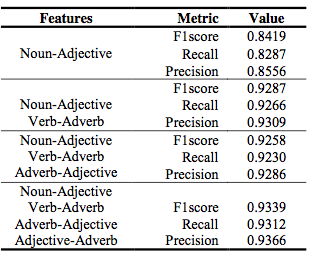
\includegraphics[width=1.0\linewidth]{tabla22.png}
\captionof{figure}{\color{Green} Clasificación con \textit{SVM}}
\end{center}\vspace{0.5cm}
\end{wrapfigure}

La segunda columna muestra en cada fila el tipo de medida y la tercera columna el valor obtenido para cada medida y para el patrón de negación correspondiente. En la Figura 2 se muestran los resultados obtenidos en la adición de cada uno de los patrones para negación léxica. Haciendo una comparación con los resultados base de la Figura 1, se observa que el único patrón que no aumentó los resultados es el que corresponde a no\textsubscript{ADVERB}-pronoun-verb. El rango de mejoras pasó de $0.41\%$ a $1.85\%$. Dos patrones superaron el $1\%$: nunca\textsubscript{ADVERB}-verb y nada\textsubscript{PRONOUN}-adjective. Nunca\textsubscript{ADVERB}-verbo apareció en $77$ opiniones positivas y $17$ opiniones negativas. Nada\textsubscript{PRONOUN}-adjective apareció en $401$ opiniones positivas y $90$ opiniones negativas.

\begin{center}\vspace{0.5cm}
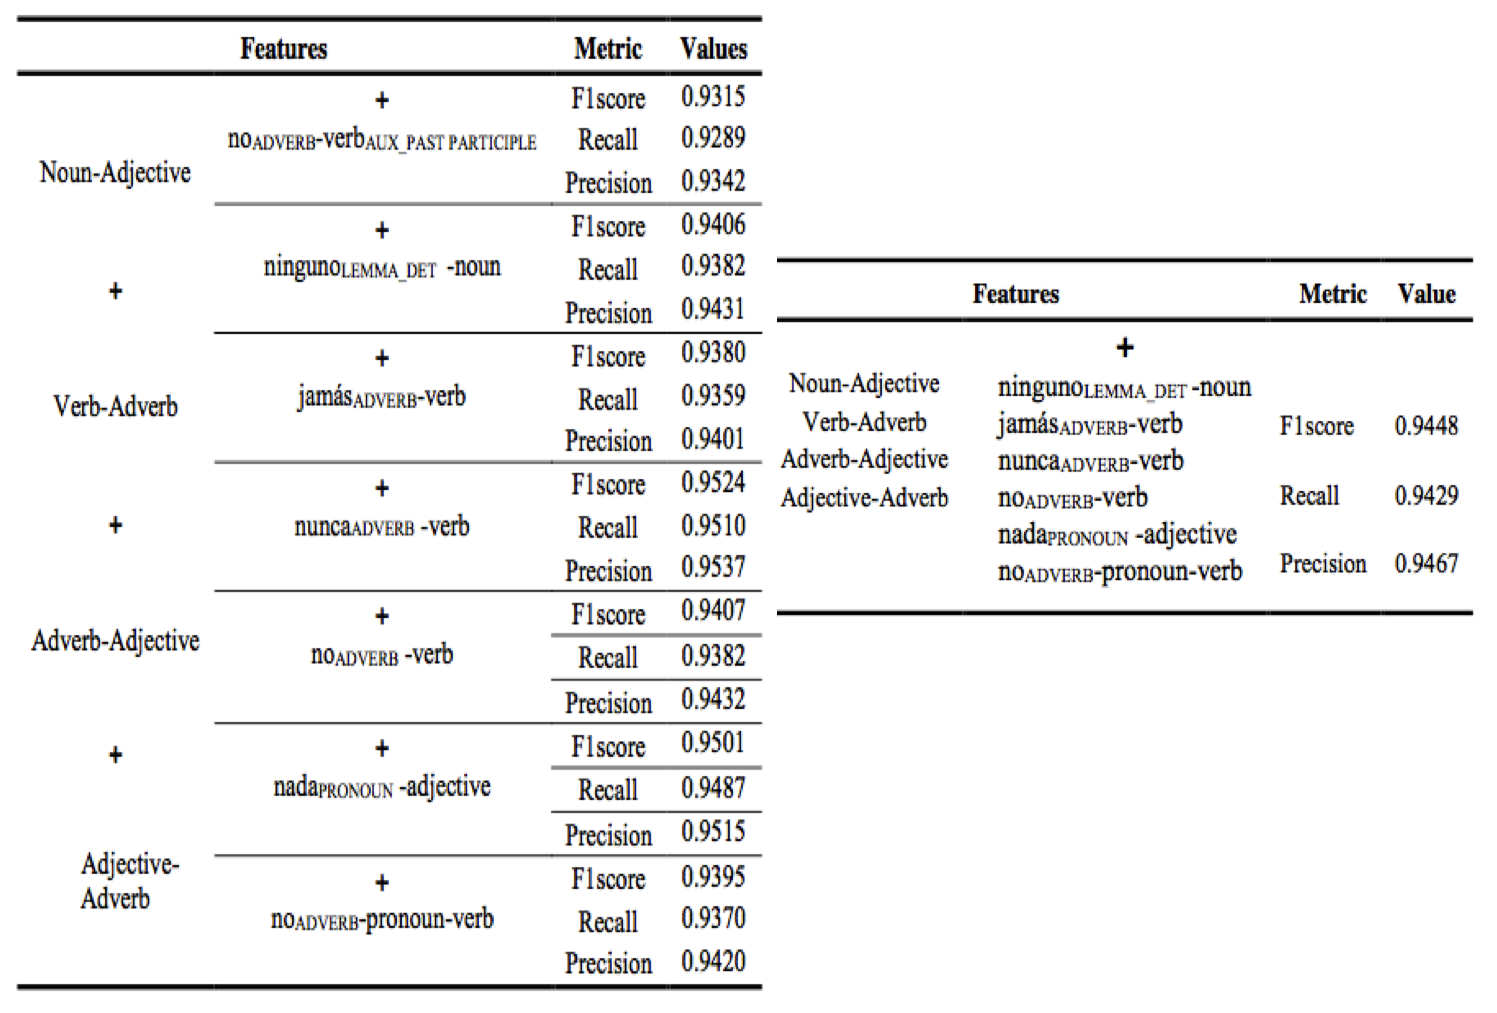
\includegraphics[width=1.0\linewidth]{tabla11.png}
\captionof{figure}{\color{Green} Rendimiento con bigramas de negación añadidos}
\end{center}\vspace{0.5cm}

Todos estos bigramas fueron usados como características de entrenamiento por el algoritmo SVM para el caso multiclase de la implementación de \textit{scikit-learn}.



%----------------------------------------------------------------------------------------
%	CONCLUSIONS
%----------------------------------------------------------------------------------------

\color{SaddleBrown} % SaddleBrown color for the conclusions to make them stand out

\section*{Conclusiones}

\begin{itemize}
\item Mostramos que usar negación léxica para generar bigramas como características del método supervisado puede ser útil para derivar la polaridad de opiniones en Español.
\item Presentamos un análisis del efecto de palabras específicas de negación para derivar la orientación semántica en opiniones en idioma Español.
\end{itemize}

\color{DarkSlateGray} % Set the color back to DarkSlateGray for the rest of the content

%----------------------------------------------------------------------------------------
%	FORTHCOMING RESEARCH
%----------------------------------------------------------------------------------------

%\section*{Forthcoming Research}

%Vivamus molestie, risus tempor vehicula mattis, libero arcu volutpat purus, sed blandit sem nibh eget turpis. Maecenas rutrum dui blandit lorem vulputate gravida. Praesent venenatis mi vel lorem tempor at varius diam sagittis. Nam eu leo id turpis interdum luctus a sed augue. Nam tellus.

 %----------------------------------------------------------------------------------------
%	REFERENCES
%----------------------------------------------------------------------------------------

\nocite{*} % Print all references regardless of whether they were cited in the poster or not
\bibliographystyle{abbrv} % Plain referencing style
\bibliography{sample} % Use the example bibliography file sample.bib

%----------------------------------------------------------------------------------------
%	ACKNOWLEDGEMENTS
%----------------------------------------------------------------------------------------

%\section*{Acknowledgements}

%Etiam fermentum, arcu ut gravida fringilla, dolor arcu laoreet justo, ut imperdiet urna arcu a arcu. Donec nec ante a dui tempus consectetur. Cras nisi turpis, dapibus sit amet mattis sed, laoreet.

%----------------------------------------------------------------------------------------

\end{multicols}
\end{document}